\documentclass[zavrsnirad]{fer}
% Dodaj opciju upload za generiranje konačne verzije koja se učitava na FERWeb
% Add the option upload to generate the final version which is uploaded to FERWeb


\usepackage{blindtext}


%--- PODACI O RADU / THESIS INFORMATION ----------------------------------------

% Naslov na engleskom jeziku / Title in English
\title{Development of an agent for solving the Entaglement game}

% Naslov na hrvatskom jeziku / Title in Croatian
\naslov{Razvoj agenta za igranje igre Entanglement}

% Broj rada / Thesis number
%\brojrada{1}

% Autor / Author
%\author{Iva Rengel}

% Mentor 
%\mentor{Prof.\@ Marko Đurasević}

% Datum rada na engleskom jeziku / Date in English
%\date{June, 2024}

% Datum rada na hrvatskom jeziku / Date in Croatian
%\datum{lipanj, 2024.}

%-------------------------------------------------------------------------------


\begin{document}


% Naslovnica se automatski generira / Titlepage is automatically generated
%\maketitle


%--- ZADATAK / THESIS ASSIGNMENT -----------------------------------------------

% Zadatak se ubacuje iz vanjske datoteke / Thesis assignment is included from external file
% Upiši ime PDF datoteke preuzete s FERWeb-a / Enter the filename of the PDF downloaded from FERWeb
% \zadatak{hr010809967773.pdf}


%--- ZAHVALE / ACKNOWLEDGMENT --------------------------------------------------

\begin{zahvale}
  % Ovdje upišite zahvale / Write in the acknowledgment
  Zahvale odličnom mentoru, Marku Đuraseviću, na potpori i pomoći u izradi završnog zarada. Zahvale Robiju, što me slušao kako meljem svaki put dok bi moje neuronske mreže postizale bolji rezultat. Hvala i mojoj obitelji, što su me podržavali tijekom izrade rada. 
\end{zahvale}


% Odovud započinje numeriranje stranica / Page numbering starts from here
\mainmatter


% Sadržaj se automatski generira / Table of contents is automatically generated
\tableofcontents


%--- UVOD / INTRODUCTION -------------------------------------------------------
\chapter{Uvod}
\label{pog:uvod}



Igru Entanglement lako je naći upisivanjem njezinog imena u internet tražilicu, ali nije je lako dobro odigrati. Naime, radi se o postavljanju manjih pločica s obrascima konca u veću sliku, gdje što zapetljanije krajnje stanje igre izgleda, to je bolji konačni rezultat. Ovaj rad istražit će kako naučiti računalni program da odigra ovu igru što je bolje moguće.

Postoje neka pravila koja su ljudskom igraču intuitivna, dok ih računalo nije svjesno. Izbjegavanje zida vodi većem rezultatu i sprječava prerani završetak igre. Konfiguriranje pločica tako da se ne prati samo glavni konac, već da se obrati pozornost i na spajanje ostalih konaca u pločici kroz koje će glavni možda proći kasnije. Ispunjavanje ploče što je moguće više, te što češće vraćanje kroz već postavljene pločice. 

Cilj ovog rada jest izrada heuristika temeljenih na nekim takvim pravilima, ali također, izrada agenta korištenjem umjetne neuronske mreže koji će moči sam sebe naučiti efikasno igrati igru, u cilju dostizanja što je moguće većeg ukupnog rezultata koji će nadmašiti čovjekov.



%-------------------------------------------------------------------------------
\chapter{Objašnjenja pojmova}
\label{pog:glavni_dio}

\section{O igri Entanglement}
\label{pog:o_igri}


Igra Entanglement jest online igra koju su napravili Gopherwood Studios \cite{gopherwoodstudios}. Igra se sastoji od velike igrače ploče s heksagonalnim izrezima u koje se postavljaju pločice. Igra kreče od središnje, već postavljene pločice. Na njoj je vidljiv "konac" izrazite boje, ovdje crven te će u kasnijim primjerima biti žarko zelen.

\begin{figure}[htb]
	\centering
	\includegraphics[width=0.58\linewidth]{Figures/game.png} 
	\caption{Prikaz originalne igre u tijeku}
	\label{slk:game_screen}
\end{figure}

Jedan potez igre jest jedno postavljanje nove pločice. Sve pločice na sebi imaju 12 smjerova, spojenih međusobno u šest nasumično izabranih puteva. Prije no što se pločica postavi na ploču, moguće ju je rotirati ili zamijeniti sa zamjenskom pločicom. Nakon postavljanja, iz onog smjera iz kojeg dolazi konac iz prijašnje ploče, put koji počinje tim smjerom bit će osvijetljen bojom. Igra se nastavlja davanjem igraču novogeneriranu pločicu koje sada može postaviti na polje gdje put konca završava.

Ako put konca ne završi u praznom polju, već u startnom polju ili na granici, igra završava. Ako put konca završava tamo gdje se nalazi već postavljena igračeva pločica, za svaku naknadnu pločicu koju konac prođe do sljedećeg praznog mjesta ili granice dodaje se linearno rastući broj bodova na vrijednost ukupnih bodova. Na primjer, ako se konac pronađe u praznom polju odmah nakon postavljanja ploče, igrač dobiva samo 1 bod. Ali ako se kraj konca pronađe na ulazu u neku drugu ploču te sveukupno prolazi kroz 4 pločice dok ne dođe do praznog polja, na kraju prolaska na vrijednost ukupnih bodova akumulirat će se 1 + 2 + 3 + 4 = 10 bodova.

\begin{figure}[htb]
	\centering
	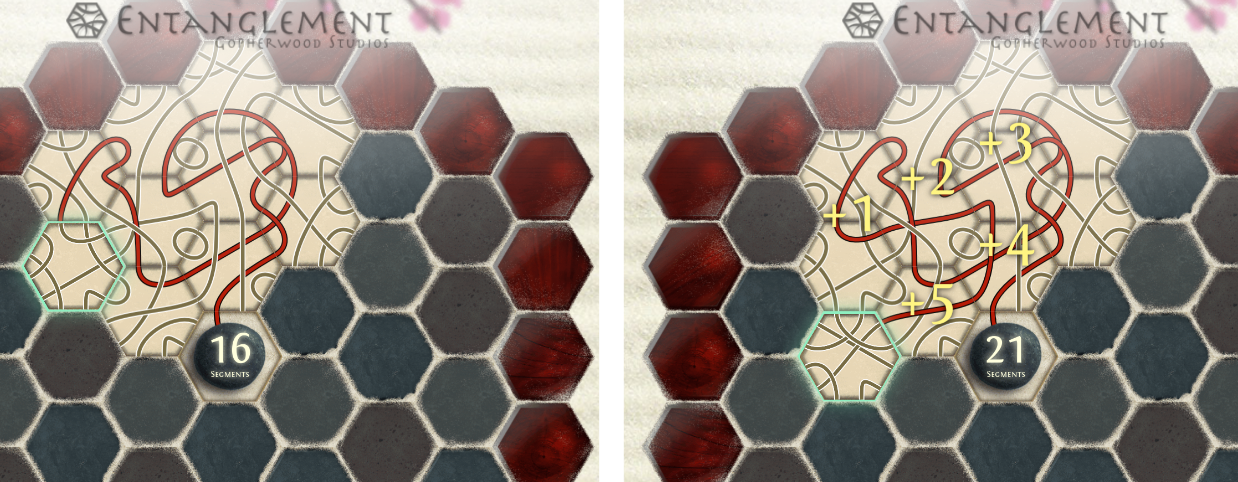
\includegraphics[width=0.78\linewidth]{Figures/scoring.png} 
	\caption{Primjer izračunavanja broja bodova za jedan korak; lijevo je ploča prije postavljanja koraka, desno nakon.}
	\label{slk:scoring}
\end{figure}

Jednom kada se trenutna pločica zamjeni sa zamjenskom, tamo će ostati do sljedeće zamjene. Cilj igre jest skupiti što je moguće više bodova prije no što se popune sve prazne pločice ili se konac "zabije" u neku od granica. U oba slučaja, krajnji bodovi isti su sveukupnim do tada akumuliranim bodovima kroz igru. Trenutno najveći broj bodova ikad sakupljen jest 5403.

\begin{figure}[htb]
	\centering
	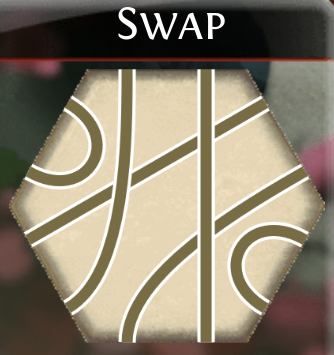
\includegraphics[width=0.2\linewidth]{Figures/zamjenska.png} 
	\caption{Zamjenska pločica, u donjem lijevom kutu prozora}
	\label{slk:swap_tile}
\end{figure}

\section{Agent umjetne inteligencije}
\label{pog:agent}
Agent u pogledu strojnog učenja jest program koji interaktira s našom igrom, od nje dobiva, skuplja i pamti informacije, te na temelju njih odlučuje koji korak će sljedeće izvršiti. Informacije koje od igre dobiva su stanja ploče prije svakog koraka, te nakon izvršenja poteza koliko bodova je bio vrijedan izvršeni potez.

Promotrit ćemo dvije temeljne vrste agenata; Oni koji biraju sljedeći potez na temelju samo trenutno dobivenog stanja i priloženim skupom pravila (heuristike). Te onaj koji o sljedećem potezu odlučuje na temelju na svim do sad sakupljenim stanjima i rezultatima, te sam definira funkcije po kojima će izabrati sljedeći korak (umjetne neuronske mreže). 

\section{Heuristike}
\label{pog:opis_heuristika}


Heuristika ili heuristička tehnika u pogledu programiranja predstavlja korištenje neke metode ili algoritma za izračun koliko je dobro koje stanje igre, te nam tako pomaže kod odabira najboljeg poteza. Ta metoda ili algoritam ne mora u svakom slučaju dati najbolji rezultat, te njen izračun ne mora imati nužno logičko objašnjenje zašto se koristi. Dovoljno je samo da nam ubrzala proces traženja sljedećih poteza ili pridonosi većem ukupnom broju bodova na kraju igre.

U pogledu na promatranu igru entanglement lako se mogu odrediti svojstva poteza o kojima ovisi rezultat igre, te će kasnije u tekstu biti razmatrane heuristike temeljene na istima. Takva promatrana svojstva su nalazi li se zid na nekom od mogućih puteva pločice koju trenutno postavljamo, koliki dug lanac dobijemo na nekom putu, te kolika je popunjenost ploče. 



\section{Umjetne neuronske mreže}
\label{pog:opis_neuronskih}

Kako bi agent mogao sam na temelju obrađenih sakupljenih podataka mogao donositi najbolje odluke bez unaprijed zadanih pravila, na neki način more biti u stanju učiti na temelju podataka. Za takvo učenje koriste se umjetne neuronske mreže. Izgrađene na temelju rada ljudskih neurona, jedan umjetni neuron uzima varijable na ulazu, te nad njima obavlja neku funkciju. Iz izlaza neurona računa se sljedeći potez igre, te se varijable funkcije neurona mijenjaju i ispravljaju nakon svake završene igre na temelju do tad sakupljenih podataka, tako da se teži najboljem rezultatu. 

Umjetna neuronska mreža skupina je takvih međusobno povezanih umjetnih neurona. Povezujemo ih u različite slojeve, gdje se prvi takvi naziva ulazni sloj, zadnji izlazni, te, oni koji su između, skriveni. Nakon svake dovršene igre svaki neuron mijenja vrijednosti svojih funkcija kako bi dobio što bolji rezultat u budućnosti. Primjer jedne umjetne mreže s dva skrivena sloja nalazi se na slici \ref{slk:prikaz_neuronske}. Oznakama 'x' označavat ću ulaze, a 'y' izlaze neuronske mreže. Broj neurona u svakom sloju jest proizvoljan.

\begin{figure}[htb]
	\centering
	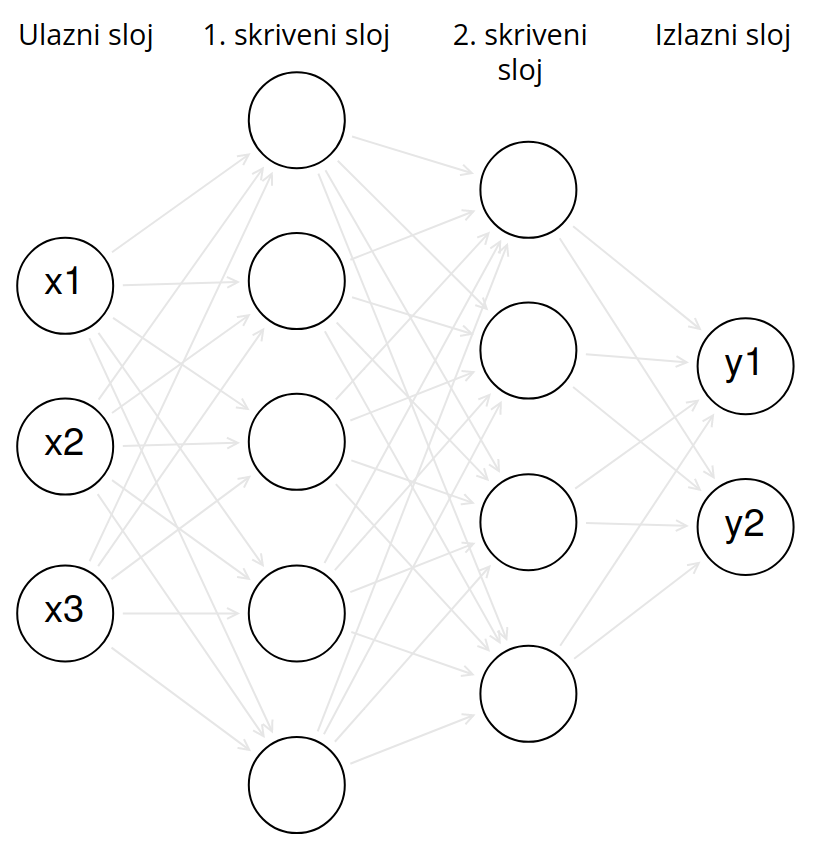
\includegraphics[width=0.58\linewidth]{Figures/neural.png} 
	\caption{Primjer umjetne neuronske mreže}
	\label{slk:prikaz_neuronske}
\end{figure}


\chapter{Pojedinosti implementacije}
\label{pog:glavni_dio2}

\section{Razvojno okruženje za implementaciju agenata}
\label{pog:razvojno_okruzenje}


Razvojno okruženje porebno za razvijanje agenata mora biti lako dostupan i izmjenjiv kod igre na koji se agent može priključiti. Naime, kod originalne online verzije igre jest skriven te je to nemoguće. Potreban je izvorni kod igre s istim pravilima. Takav je pronađen u GitHub repozitoriju \cite{entanglementgithub} entanglement osobe Brian Shaginaw.

Ovaj repozitorij pisan je u Pythonu 2, pa je prva stvar kod spajanja na izvorni kod bila mijenjanje i prilagođavanje koda da radi s Pythonom verzije 3. Ovaj korak izveden je relativno brzo, te je sljedeći dio zauzeo puno više vremena, a to je proučavanje i pokušavanje spajanja na kod te istraživanje što su to heuristike i kako ih uspješno implementirati. Igra jest klasa koju će agent kasnije pozivati.

\begin{figure}[htb]
	\centering
	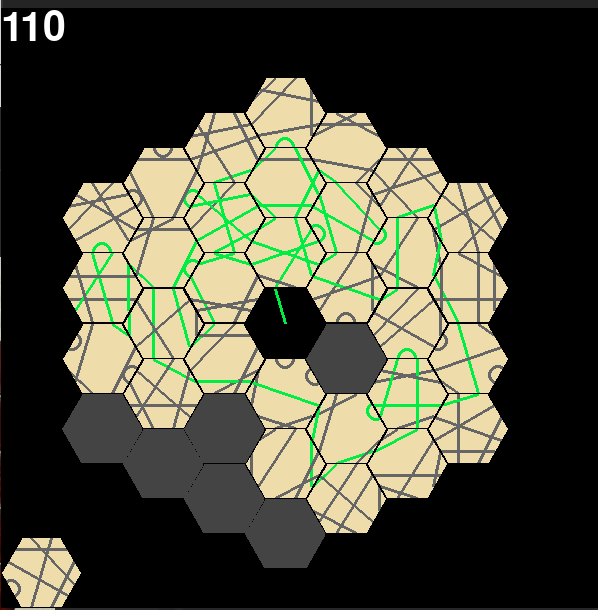
\includegraphics[width=0.58\linewidth]{Figures/gamefinished.png} 
	\caption{Prikaz preuzete igre}
	\label{slk:game_finished}
\end{figure}

U kod je bilo potrebno dodati neke nove funkcije. Radi preglednosti i otkrivanja pogrešaka, implementirane su funkcionalnosti pauziranja i izlaska iz programa. Dodana je metoda resetiranja igre, kako bi se, nakon zabijanja konca u zid, umjesto da program završi s radom umjesto toga obrisala ploča, spremili rezultati te započela nova runda igre. Također, dodana je metoda koja na temelju ulaza obavlja jedan korak igre (postavljanje pločice).



\section{Definicija stanja igre, ploče, opasnosti i koraka}
\label{pog:definicija_stanja}

Kako bismo mogli birati optimalne korake od onih mogućih, nekako moramo definirati koliko nam je svaki korak vrijedan. Vrijednost koraka ovisit će o trenutnom stanju igre. Naime, pločica se ne nalazi u istoj situaciji ako je okružena praznim poljima, ili ako je samo jedno neposredno mjesto uz nju prazno. Zato moramo prikupiti informacije iz izgleda same ploče u neku strukturu koju će nam biti lakše obraditi.

Stanje igre temeljit ćemo na već postojećim tipu podataka u kodu nazvanoj Board, što je klasa koja predstavlja igraću ploču (Slika \ref{slk:class_diagram}).

\begin{figure}[htb]
	\centering
	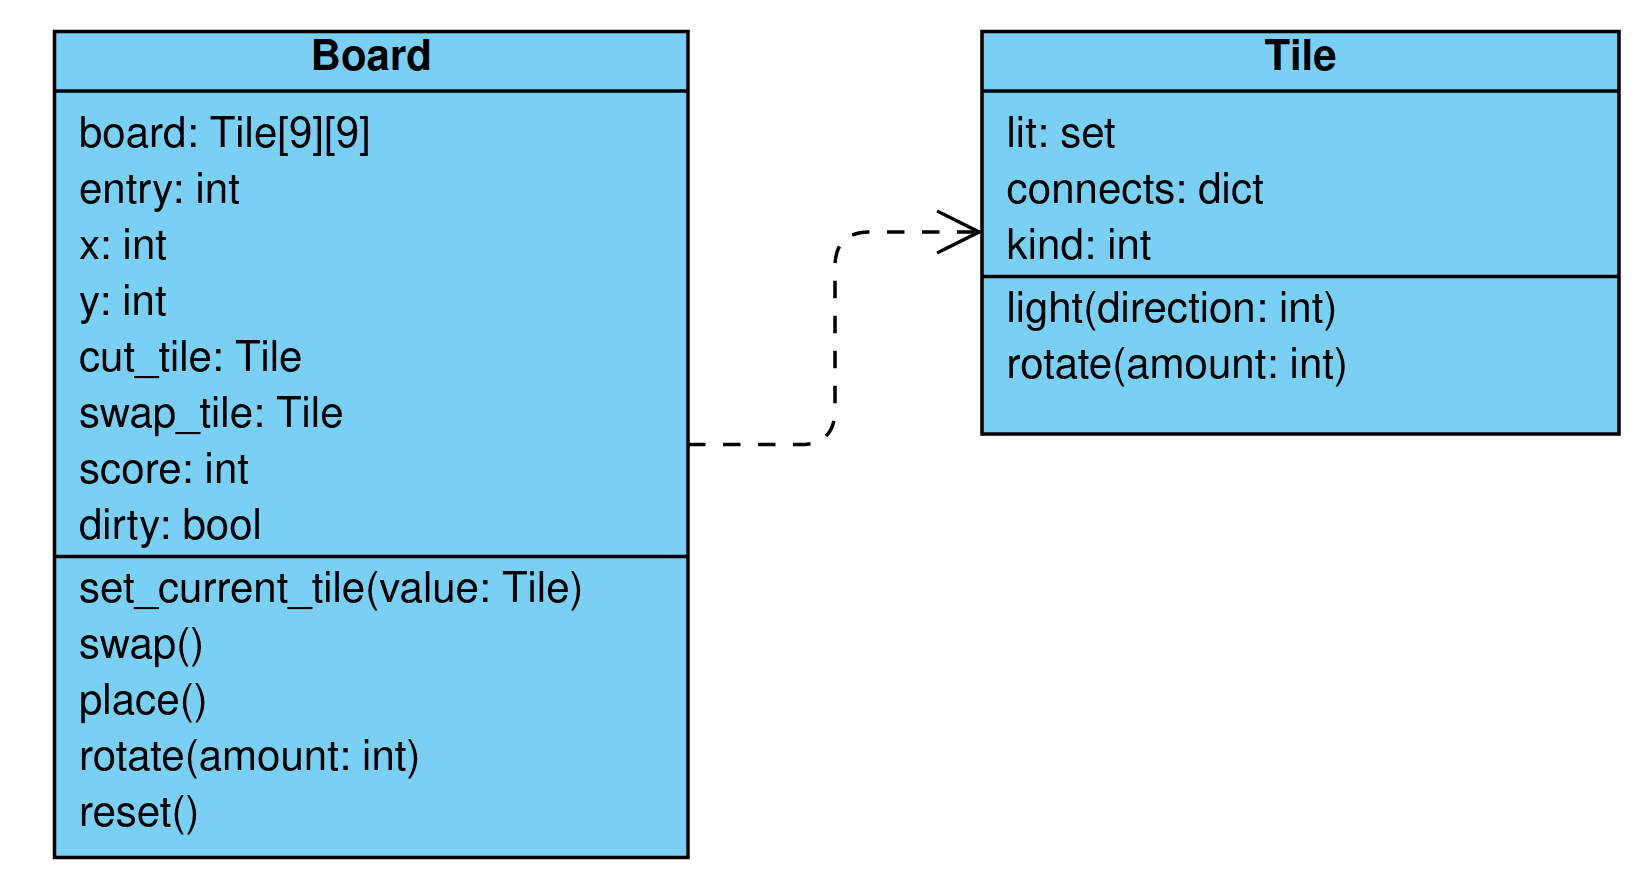
\includegraphics[width=0.68\linewidth]{Figures/board_diagram.png} 
	\caption{Dijagram razreda Board i Tile}
	\label{slk:class_diagram}
\end{figure}

Unutar te klase imamo mnoštvo atributa:
\begin{itemize}
	\item \textbf{board} lista svih pločica, te svaka od njih pamti svoju vrstu (otvorena, zatvorena, start-pločica ili igraća), te ako je igraća, izgled svojih konaca i par osvijetljenih konaca
	\item \textbf{entry} iz kojeg od 12 smjerova na pločicu koja se trenutno postavlja dolazi osvijetljeni konac
	\item \textbf{x i y} koordinate pločice koja se trenutno postavlja
	\item \textbf{curr tile} trenutna pločica
	\item \textbf{swap tile} zamjenska pločica
	\item \textbf{score} do sad skupljeni broj bodova
	\item \textbf{dirty} je li igra započeta, je li ikoja pločica postavljena na ploču.
\end{itemize}

Stanje igre jest dugo polje cjelobrojnih varijabli izračunatih uz pomoć ploče igre. Za svaki od 12 smjerova one pločice na koje trenutne koordinate pokazuju, izračunava se duljina puta do sljedećeg praznog mjesta (0 ako je to mjesto odmah susjedno trenutnim koordinatama, 1 ili više ako prvo vodi kroz već postavljene ploče prije praznog mjesta), je li taj smjer opasan ili ne, koje su koordinate praznog polja na kojem će završiti, koji su smjerovi već izgeneriranih trenutne i zamjenske pločice. Različito stanje igre jest potrebno za različite heuristike, te će kasnije kod opisa svake biti objašnjena i struktura polja stanja igre.

Opasnost definiramo kao onaj potez koji dovodi do kraja igre. Od četiri moguća tipa pločica, zatvorena i start-pločica su opasne i kad vrh konca dođe do njih igra završava. Ako bi potez vodio konac na neki smjer koji pokazuje na igraću pločicu, potrebno je rekurzivnim algoritmom odrediti u kojem tipu pločice se nalazi njegov završetak. Tada možemo odrediti je li taj smjer opasan ili ne.

Jedan korak, ili jedan potez, sastoji se od postavljanjem ili nepostavljanjem zastavice za mijenjanje trenutne pločice sa zamjenskom, te rotiranja izabrane u smjeru kazaljke na satu za neki cjelobrojni broj od 0 do 5. To nam daje ukupno 12 različitih mogućnosti za svaki korak.

\chapter{Razrada heuristika}
\label{pog:razrada_heuristika}

\section{Biranje koraka slučajnim odabirom}
\label{pog:slucajan_odabir}

Kako bismo imali nešto s čime dalje možemo uspoređivati efektivnost koje heuristike pogledat ćemo što se događa s igrom ako joj prepustimo odabir svakog sljedećeg koraka slučajnom odabiru. Nakon 100 koraka igre, vidljivo je da se rezultat kreće oko 9 bodova na grafu priloženom na slici \ref{slk:random_graph}.


\begin{figure}[htb]
	\centering
	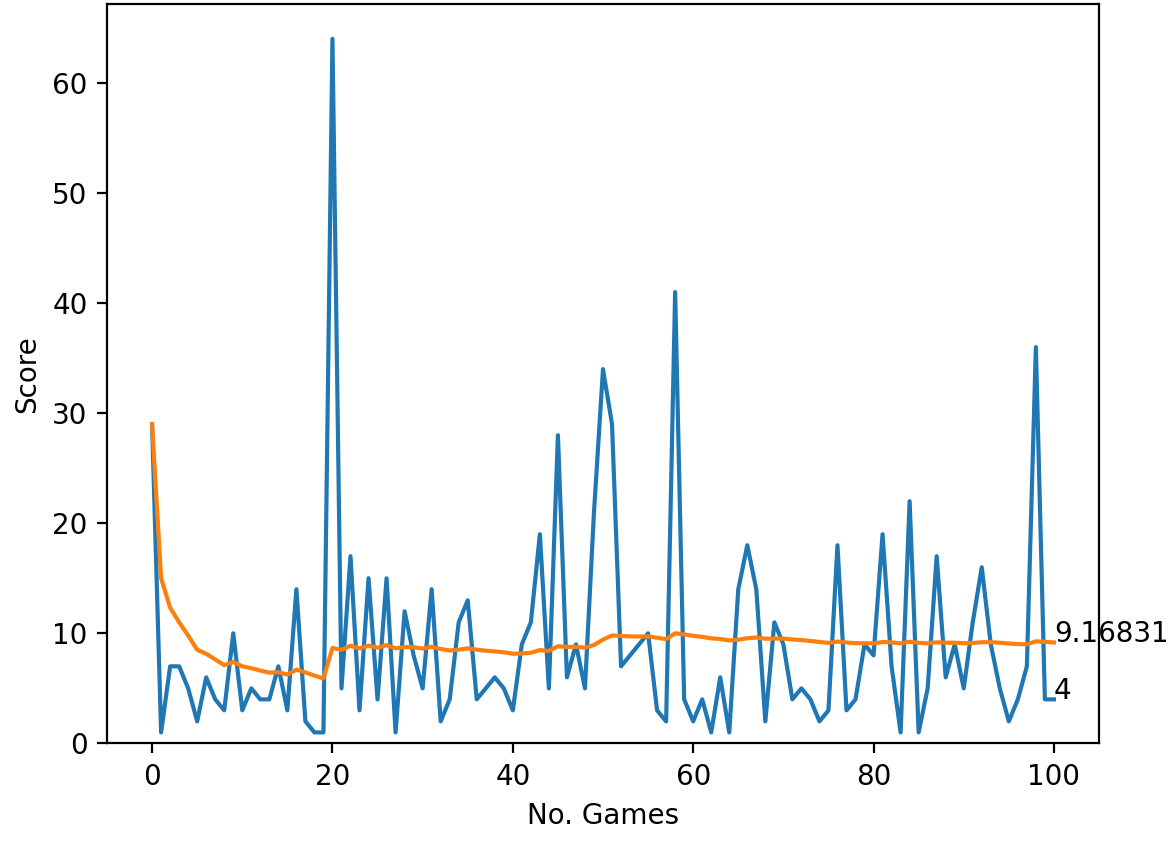
\includegraphics[width=0.58\linewidth]{Figures/random.png} 
	\caption{Graf slučajnog odabira poteza nakon 100 instanci igre}
	\label{slk:random_graph}
\end{figure}

\section{Neposredna heuristika}
\label{pog:neposredna}

Prva heuristika koju promatramo stanje igre izračunava kao polje od svega šest cjelobrojnih vrijednosti. Svaka varijabla poprima vrijednost 0 ili 1, gdje nula označava da je taj smjer neposredno siguran, te jedinica označava da nije. Ako se neposredno od trenutne pločice pojavi već postavljena pločica, heuristika je smatra sigurnom. Zbog toga program u često mnogo slučajeva završi prije nego što popuni cijelu ploču.

Igra računa sljedeći potez tako da slučajnim odabirom izabere za koliko će se rotirati trenutna pločica, te provjeri je ti takav potez opasan. Ako je, izračunava se novi potez, te ako su svi potezi nesigurni, mijenja se trenutna pločica sa zamjenskom. Ovakva heuristika pridonosi rezultatu od prosječno 25 bodova, vidljivo na slici \ref{slk:sofort_graph}

\begin{figure}[htb]
	\centering
	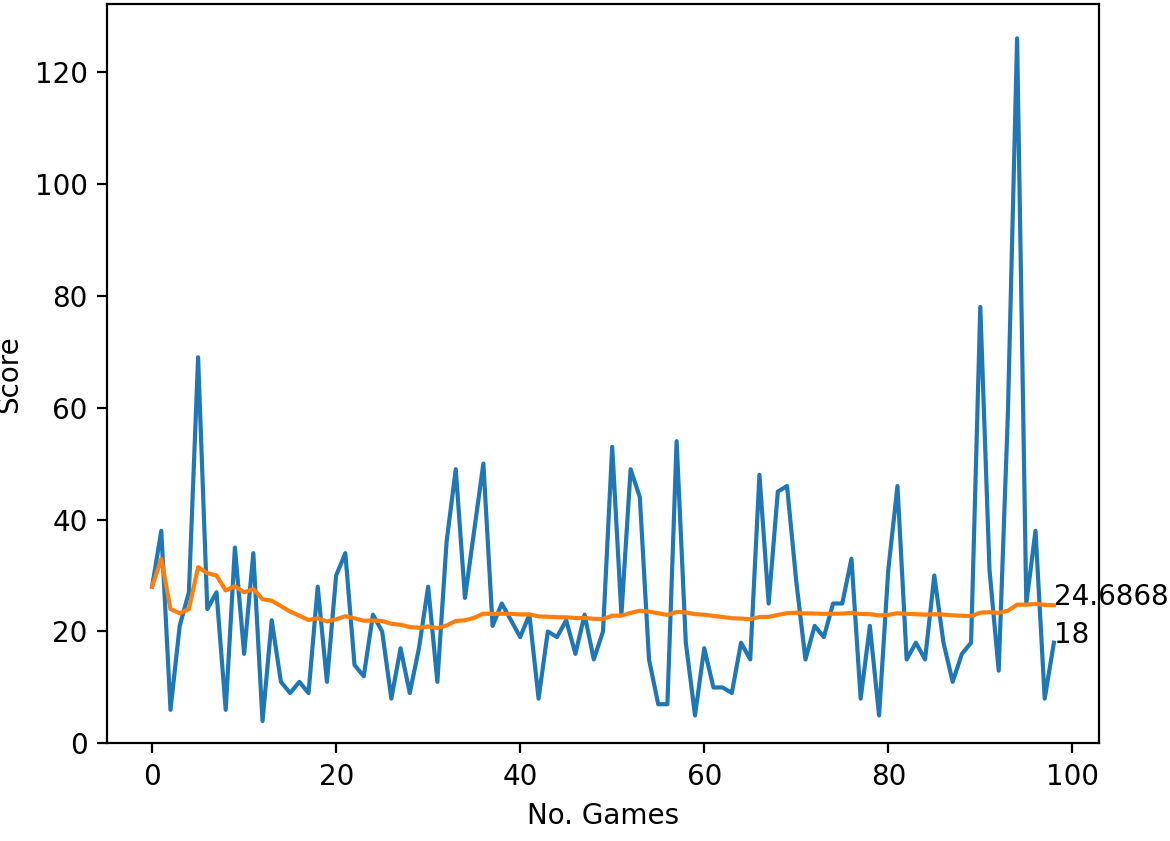
\includegraphics[width=0.58\linewidth]{Figures/sofort.png} 
	\caption{Graf neposredne heuristike nakon 100 instanci igre}
	\label{slk:sofort_graph}
\end{figure}


\section{Dubinska heuristika sa slučajnim odabirom}
\label{pog:dubinska_slucajna}

S ovom heuristikom proširujem stanje igre na izračunavanje vode li i već postavljene igraće ploče u opasnost. Odabir poteza radi na isti način kao i u prijašnjem orimjeru, te se sad prosječan broj bodova podigao na čak 75 te se ploča u većini slučajeva popuni barem 80 posto [Slika \ref{slk:reach_graph}].

\begin{figure}[htb]
	\centering
	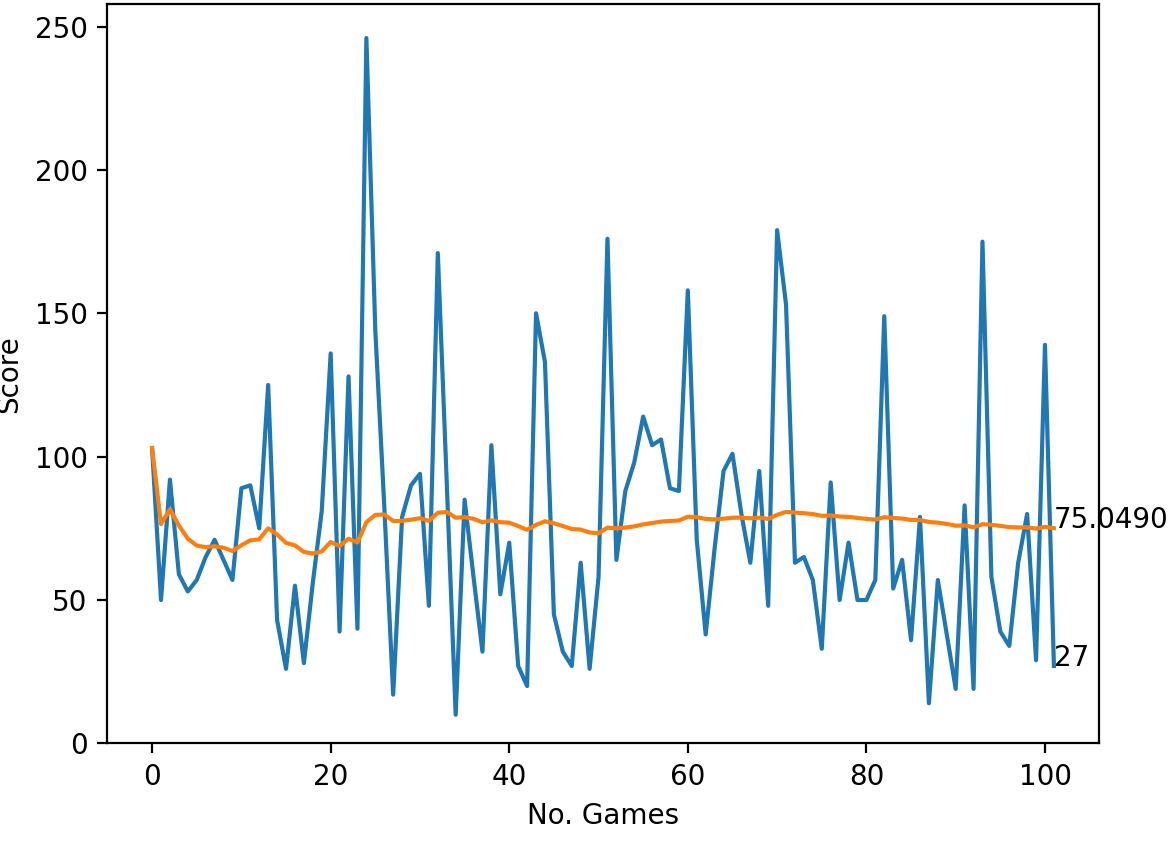
\includegraphics[width=0.58\linewidth]{Figures/reach.png} 
	\caption{Graf dubinske heuristike (slučajne) nakon 100 instanci igre}
	\label{slk:reach_graph}
\end{figure}


\section{Dubinska heuristika s izračunavanjem najduljeg puta}
\label{pog:dubinska}

Umjesto da bira potez slučajnim odabirom, ova heuristika prolazi kroz sve puteve koje je moguće doseći sa trenutnom i zamjenskom pločicom te od njih uzima onaj koji pridonosi najviše bodova instanci igre. Prosjek sakupljenih upupnih bodova sada je 91 [Slika \ref{slk:depth_graph}].

\begin{figure}[htb]
	\centering
	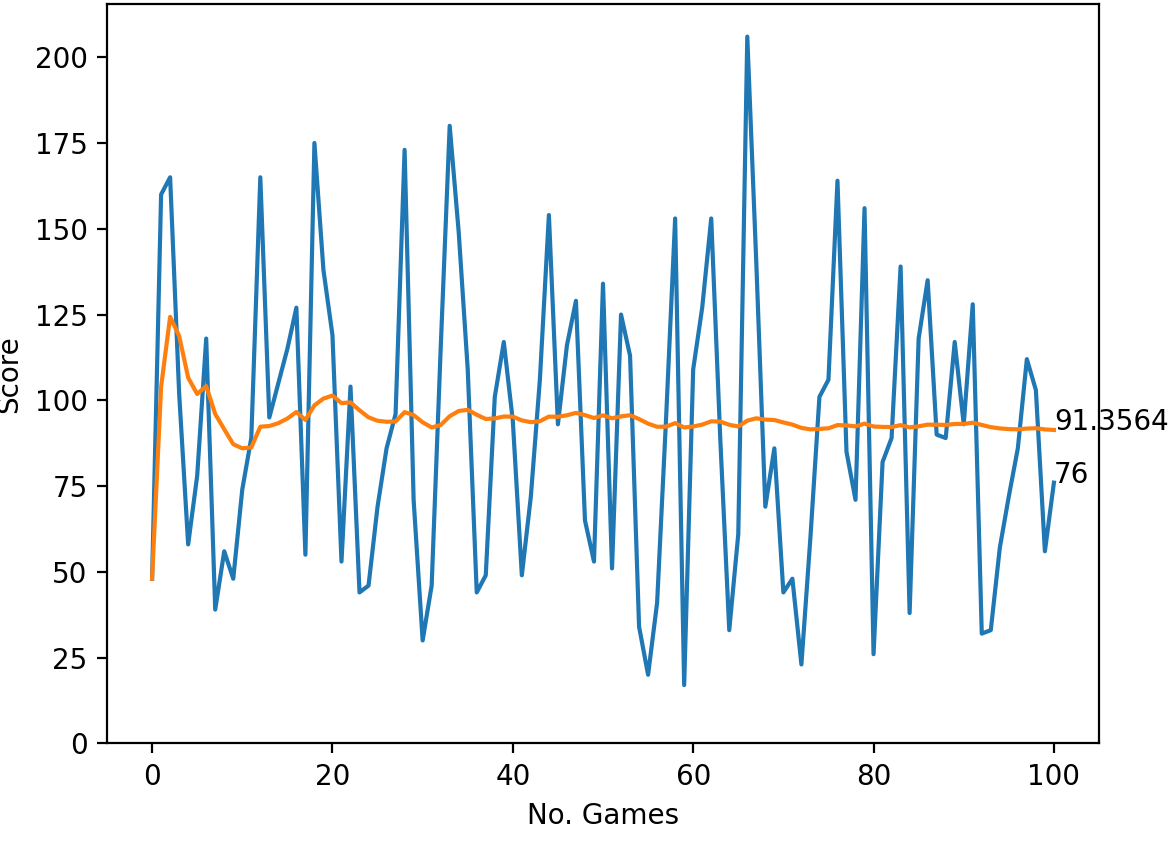
\includegraphics[width=0.58\linewidth]{Figures/depth.png} 
	\caption{Graf dubinske heuristike nakon 100 instanci igre}
	\label{slk:depth_graph}
\end{figure}


\chapter{Razrada umjetnih neuronskih mreža}
\label{pog:razrada_neuronske}

Razlika između agenta s heuristikom i onog s umjetnom neuronskom mrežom koju naziremo iz samih grafova jest razlika u prosječnim rezultatima igre kroz vrijeme. Dok se heuristike oslanjaju samo na statička pravila, svaku igru odigraju relativno podjednako dobro, te je njihov prosječni rezultat teži u isti broj bez obzira koliko instanci igre promatramo. U drugu ruku, umjetna neuronska mreža uči kroz vrijeme, te tako i njezin prosječni rezultat raste sa brojem odigranih instanci igre.

Problem na koji se nailazi kod implementacije neuronskih mreža jest optimizacija postupka učenja. Naime, veličina polja ulaza te broj neurona u mreži utječi proporcionalno na vrijeme potrebno za izučavanje neuronske mreže do željenog rezultata. Zbog toga minimiziramo navedene aspekte problema toliko dokle prosječni rezultat svih igara znatno ne opada.

\begin{table}[]
	\centering
	\begin{tabular}{|l|lll|}
		\hline
		broj neurona & jedan skriveni sloj & dva skrivena sloja & tri skrivena sloja \\ \hline
		20                                    & 243                 & 742                & \textgreater{}3000 \\
		40                                    & 388                 & 1146               & \textgreater{}3000 \\ \hline
	\end{tabular}
	\caption{Koliko instanci igara je potrebno prije nego li se postigne prosječan rezultat od 30 za različite veličine skrivenih slojeva}
	\label{tab:velicina_mreze}
\end{table}

Ako ne mijenjamo ni jedan parametar osim broja neurona u skrivenom sloju i broj tih slojeva, u tablici \ref{tab:velicina_mreze} vidimo dobivene rezultate. To jest, u tablici su zapisani brojevi instanci igre koji su bili potrebni da umjetna neuronska mreža postigne prosječan rezultat od barem 30 bodova. Vidljivo je da povećavanje broja slojeva neurona znatnije utječe na brzinu učenja mreže nego samo povećavanje broja neurona u sloju.

Još jedan problem jest veličina ulaznog polja. Što je ono veće i zamršenije, neuronskoj mreži je teže povezati informacije te iz njih zaključiti što pridonosi boljem rezultatu. Prva isprobana neuronska mreža primala je skoro cijelo stanje igre (za svaki od 12 puteva je li siguran, koliki rezultat daje, gdje će završiti kraj konca ako ode tim putem, konfiguraciju trenutne i zamjenske pločice) veličine 73 cjelobrojna broja. Rezultati navedene mreže nisu prelazili čak ni rezultat agenta koji bira sljedeći korak slučajnim odabirom satima. Čak ni nakon postupnog smanjivanja tog polja na dvadesetak ulaza, prosječni rezultati igara nisu se povećavali, što znači da se neuronska mreža nije mogla naučiti ni jednostavna pravila kao izbjegavanje zidova.



\section{Umjetna neuronska mreža s izbjegavanjem opasnosti}
\label{pog:neuronska_opasnost}
Konstruirana umjetna neuronska mreža sadrži 12 ulaznih, te isto toliko izlaznih neurona. Također u dva skrivena sloja po 20 neurona u svakom. Kao polje ulaznih vrijednosti šalje se informacija o tome je li, odabirom tog smjera, on siguran. Mogući smjerovi prikazani su u tablici \ref{tab:ulazna_polja}, s napomenom da se pločice uvijek miču u smjeru obrnutom kazaljki na satu. Izlazno polje jest polje vrijednosti 0 ili 1, i to tako da samo jedna vrijednost može biti 1. Indeks mjesta jedinice u izlaznom polju označava potez koji će se odigrati.


\begin{figure}[htb]
	\centering
	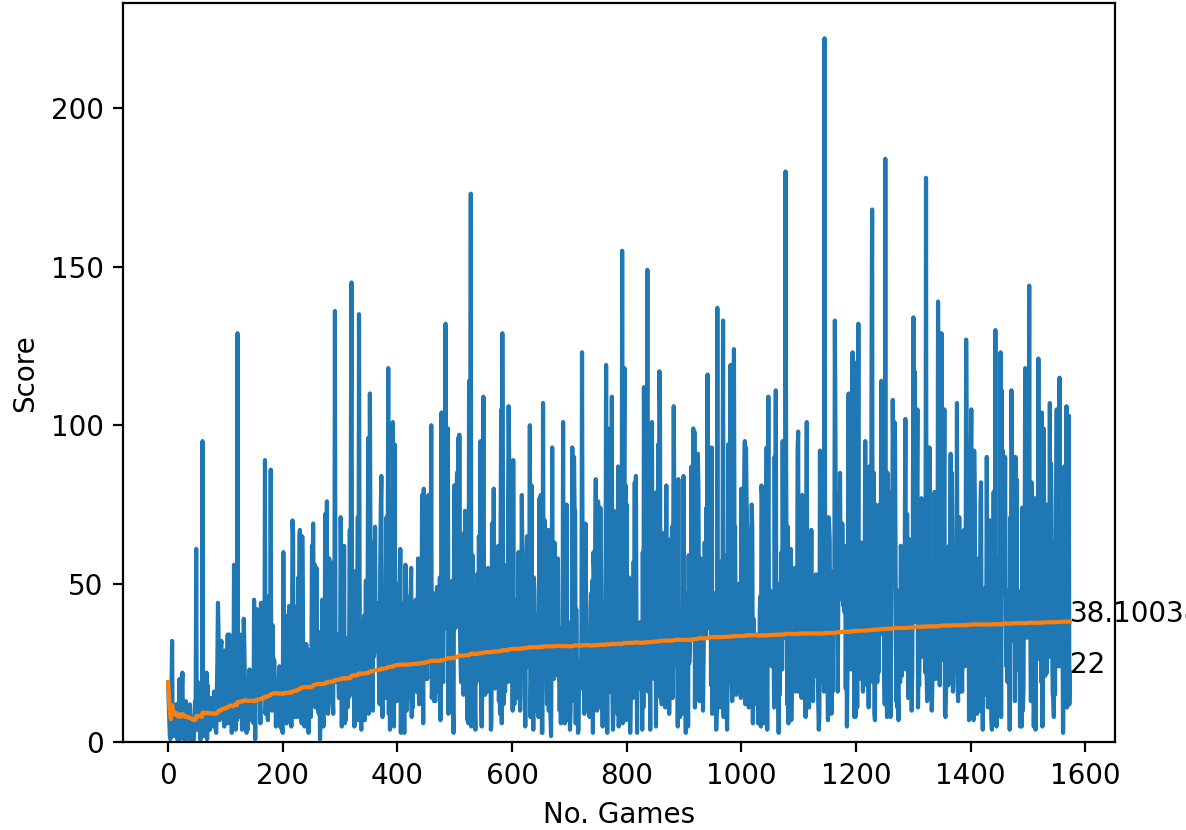
\includegraphics[width=0.58\linewidth]{Figures/neuronska1.png} 
	\caption{Graf umjetne neuronske mreže s izbjegavanjem opasnosti}
	\label{slk:neural_graph}
\end{figure}


\begin{table}[]
	\centering
	\begin{tabular}{|l|l|l|l|}
		\hline
		indeks & izlazno polje                & indeks & izlazno polje                 \\ \hline
		0      & trenutna pločica bez pomaka  & 6      & zamjenska pločica bez pomaka  \\
		1      & trenutna pločica s pomakom 1 & 7      & zamjenska pločica s pomakom 1 \\
		2      & trenutna pločica s pomakom 2 & 8      & zamjenska pločica s pomakom 2 \\
		3      & trenutna pločica s pomakom 3 & 9      & zamjenska pločica s pomakom 3 \\
		4      & trenutna pločica s pomakom 4 & 10     & zamjenska pločica s pomakom 4 \\
		5      & trenutna pločica s pomakom 5 & 11     & zamjenska pločica s pomakom 5 \\ \hline
	\end{tabular}
	\caption{Izlazno polje umjetne neuronske mreže}
	\label{tab:ulazna_polja}
\end{table}


\section{Umjetna neuronska mreža s informacijom o najduljem putu}
\label{pog:neuronska_najdulji}

Izlazno polje ostaje isto u svim neuronskim mrežama, dok ulazno mijenjamo. Umjesto slanja samo informacija je li put siguran, šalje se i informacija o tome je li taj put najdulji, to jest hoće li dati najveći rezultat. Prosječan rezultat takve neuronske mreže seže do 87 bodova [Slika \ref{slk:second_neural}].

\begin{figure}[htb]
	\centering
	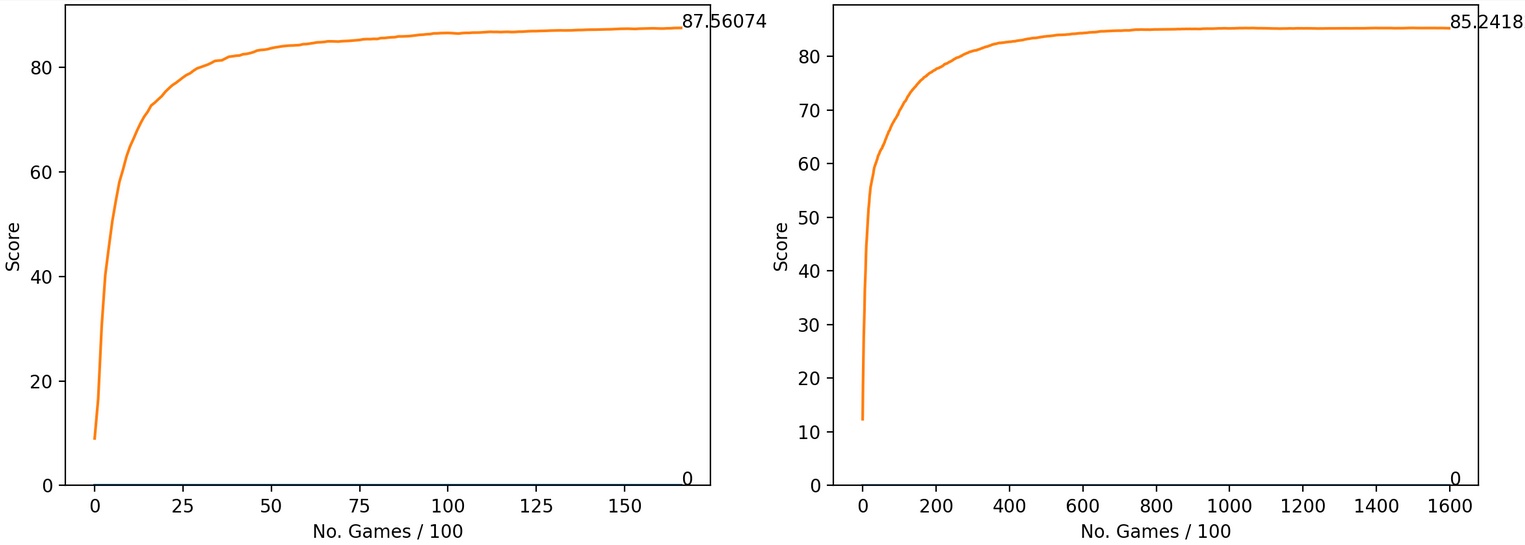
\includegraphics[width=0.88\linewidth]{Figures/neural_second.png} 
	\caption{Umjetna neuronska mreža s informacijom o najduljem putu. Lijevo, jedan skirven sloj s 20 neurona. Desno, dva sloja s 20 neurona.}
	\label{slk:second_neural}
\end{figure}

\section{Umjetna neuronska mreža s ostalim informacijama}
\label{pog:neuronska_ostale}
U ulaz, osim informacija o sigurnosti i duljini pojedinih koraka, možemo poslati i ostale informacije o igri. Šaljemo broj poteza unutar jedne igre, te poziciju pločice koja se trenutno postavlja. Rezultat takve mreže kroz vrijeme vidljiv je na slici \ref{slk:neural_meta}. 

\begin{figure}[htb]
	\centering
	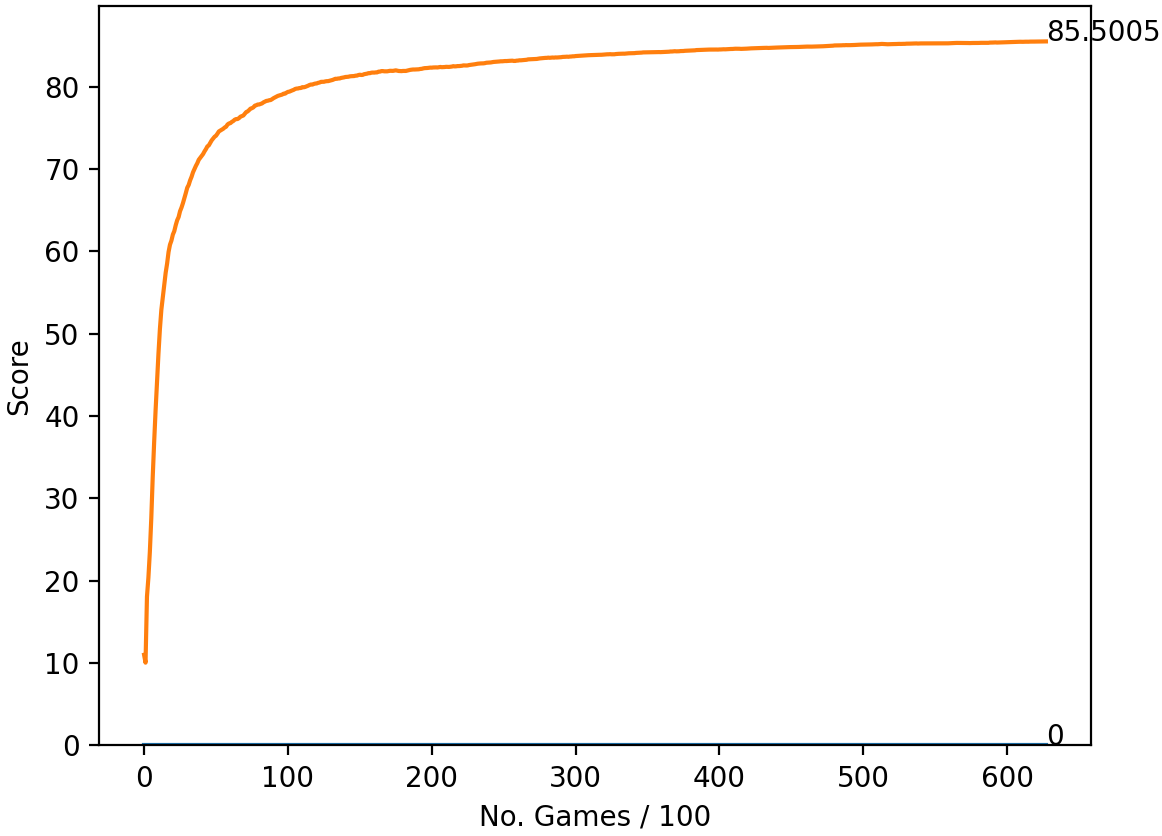
\includegraphics[width=0.58\linewidth]{Figures/dodatna.png} 
	\caption{Umjetna neuronska mreža s dodatnim rezultatima}
	\label{slk:neural_meta}
\end{figure}

Jedna strategija koja osigurava veći rezultat jest osiguravanje da se prazni konci povezani sa zidom s jedne strane, povežu sa zidom i s druge. [Slika \ref{slk:neural_loops}] To smanjuje broj potencijalno opasnih puteva u sljedećim koracima igre. Kao ulaz, osim informacija o najboljem putu, šalje se i broj puteva konca koji se vraćaju u svoj susjedni put. Ako se pločica s takvom konfiguracijom odmah postavi pokraj zida, sprječava se mogućnost zabijanja u taj isti zid u budućnosti. 

\begin{figure}[htb]
	\centering
	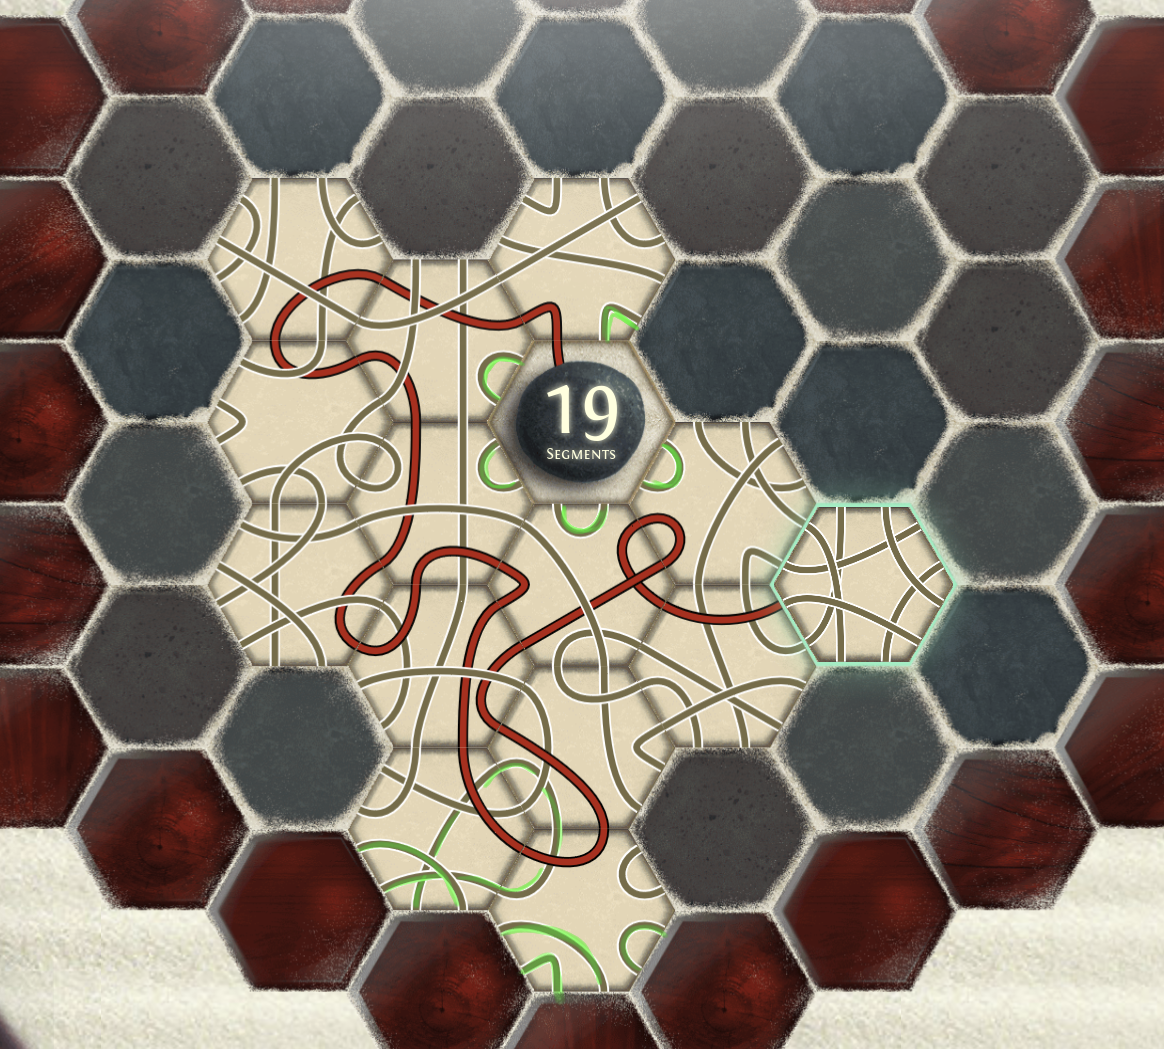
\includegraphics[width=0.48\linewidth]{Figures/loops.png} 
	\caption{Prikaz praznih konaca (zeleno) te kako su povezana sa zidovima iz obje strane}
	\label{slk:neural_loops}
\end{figure}

Umjesto da se takva informacija šalje kao poseban element ulaza, prije svakog koraka agent izračunava može li njime povezati dva zida zajedno, te ako može, za taj korak na mjestu ulaza postavlja broj 3. Dobiveni rezultat nadilazi prijašnje mreže, te joj prosječni rezultat doseže više od 93 bodova [Slika \ref{slk:neural_loops2}].

\begin{figure}[htb]
	\centering
	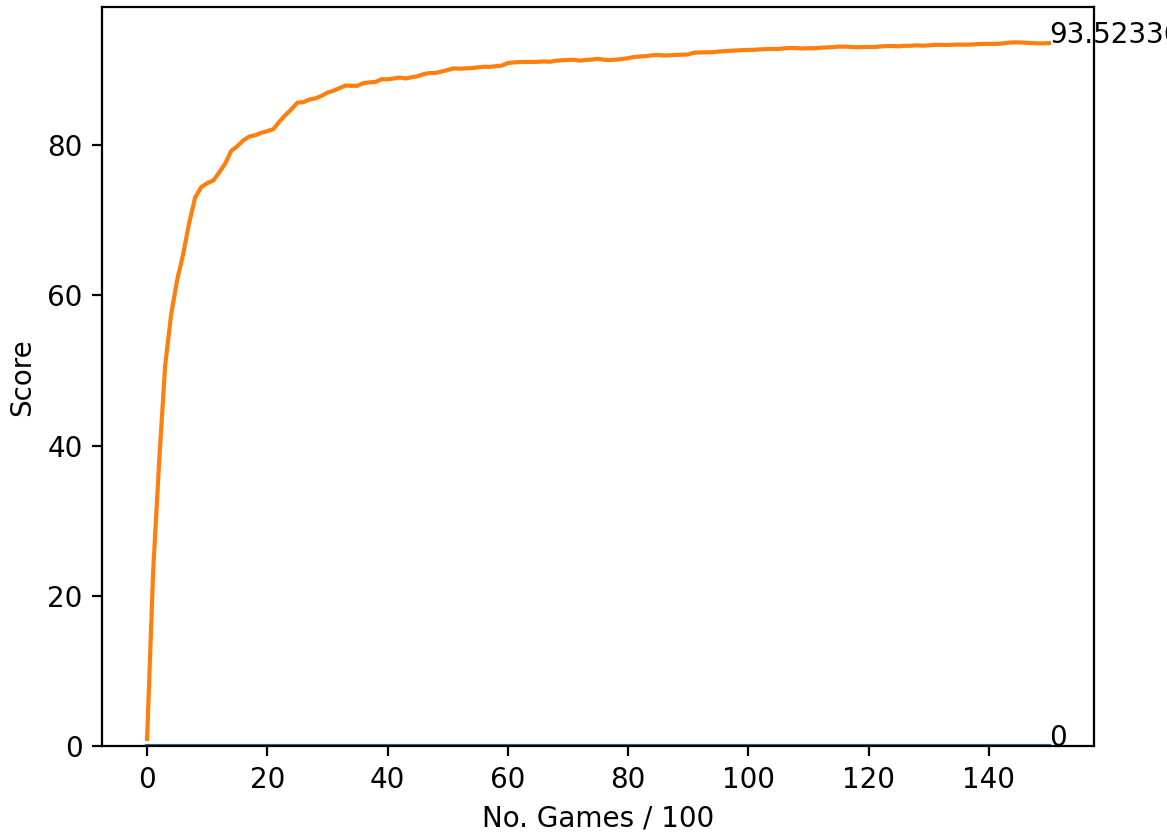
\includegraphics[width=0.58\linewidth]{Figures/loops_graph2.png} 
	\caption{Rezultat umjetne neuronske mreže s informacijom o praznim koncima}
	\label{slk:neural_loops2}
\end{figure}

Igranjem s prioritetu u ulaznom polju, doseže se još veći prosječni rezultat od preko 104 boda [Slika \ref{slk:neural_connections}]. Prioritet se računa prema sljedećem:
\begin{enumerate}
	\item Siguran potez koji spaja sve opasne puteve zajedno i daje najveći rezultat
	\item Siguran potez koji spaja neke opasne puteve zajedno i daje najveći rezultat
	\item Siguran potez koji ne spaja opasne puteve ali daje najveći rezultat
	\item Siguran potez koji spaja sve opasne puteve zajedno
	\item Siguran potez koji spaja neke opasne puteve zajedno
	\item Siguran potez koji ne spaja opasne puteve
	\item Opasan potez
\end{enumerate}

\begin{figure}[htb]
	\centering
	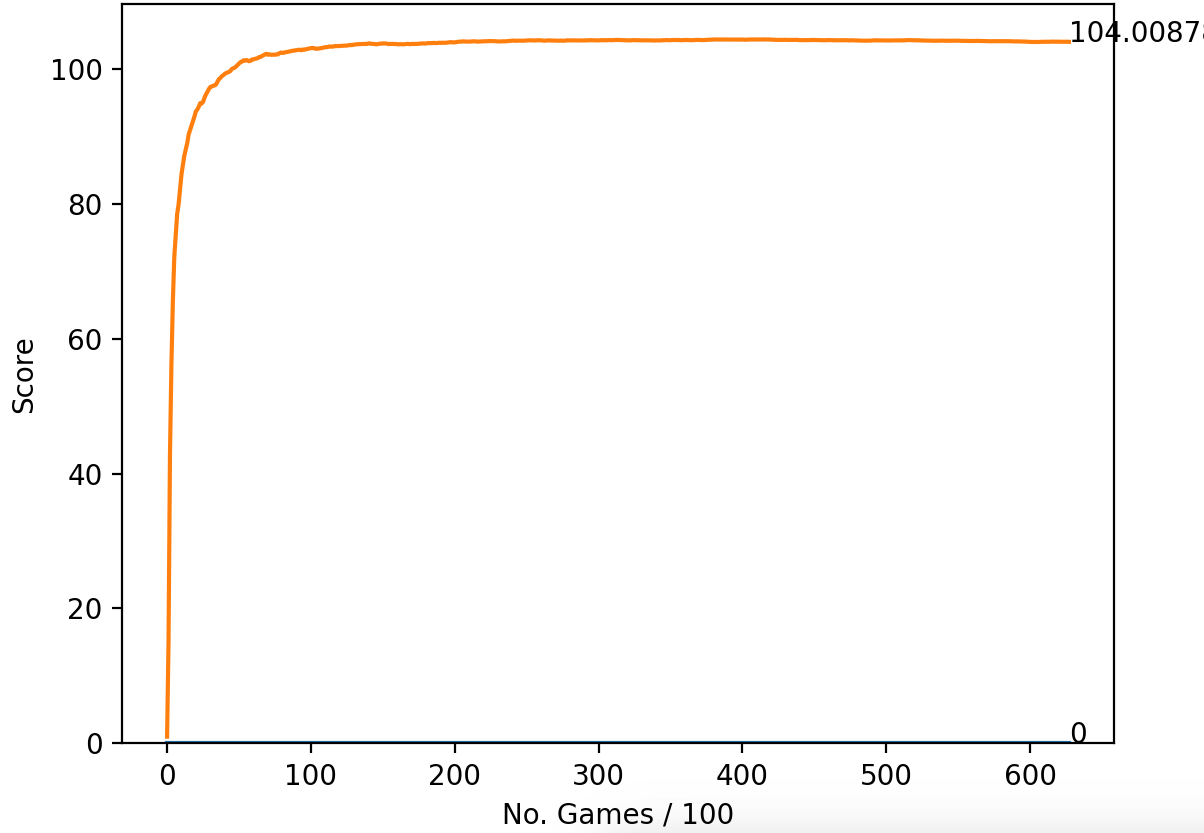
\includegraphics[width=0.58\linewidth]{Figures/najbolja.png} 
	\caption{Rezultat umjetne neuronske mreže s informacijom o praznim koncima s izmjenjenim ulaznim poljem}
	\label{slk:neural_connections}
\end{figure}

%-------------------------------------------------------------------------------
\chapter{Usporedba rezultata}
\label{pog:usporedba_rezultata}

Raspored sakupljenih bodova na kraju svake instance igre kroz 3000 odigranih rezultata usporedit će mo na grafu dubinske heuristike [Slika \ref{slk:heuristic_histograph}] i na grafu razvijene neuronske mreže s informacijom o najduljem putu [Slika \ref{slk:neural_histograph}]

\begin{figure}[htb]
	\centering
	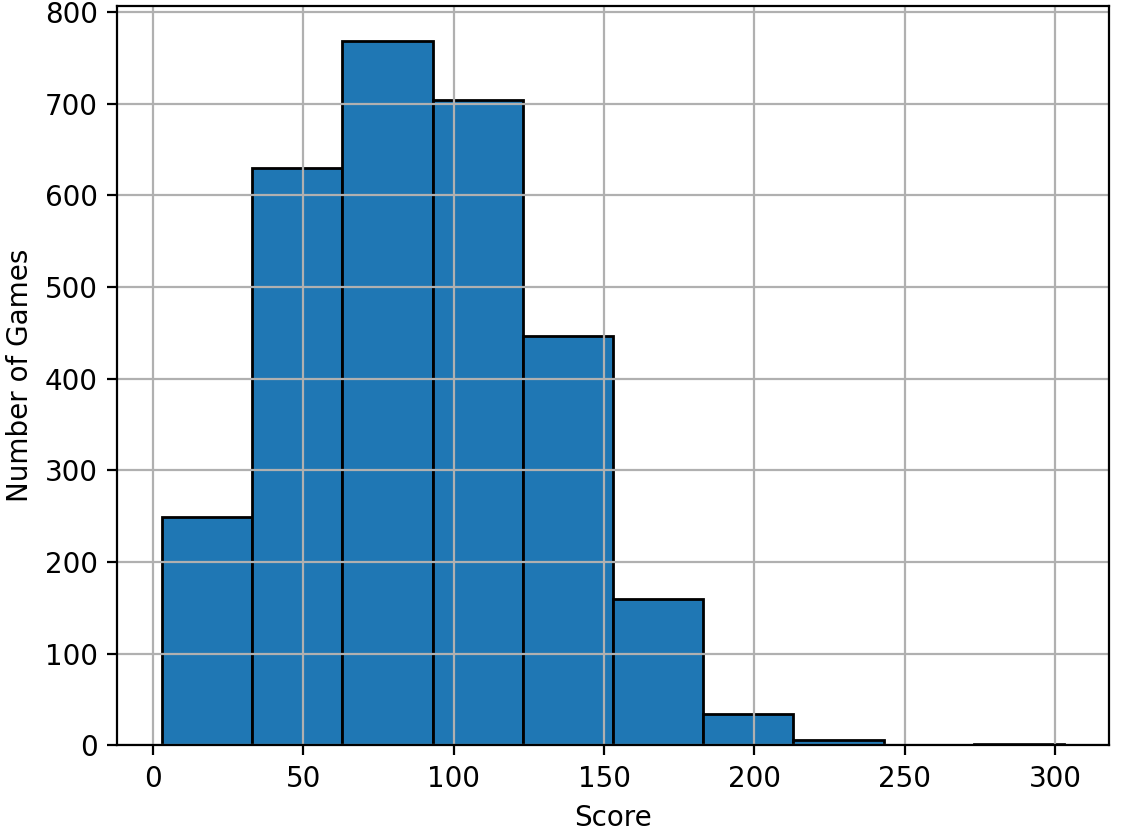
\includegraphics[width=0.58\linewidth]{Figures/histoheuristic.png} 
	\caption{Histogram rezultata dubinske heuristike kroz 3000 instanci igre}
	\label{slk:heuristic_histograph}
\end{figure}

\begin{figure}[htb]
	\centering
	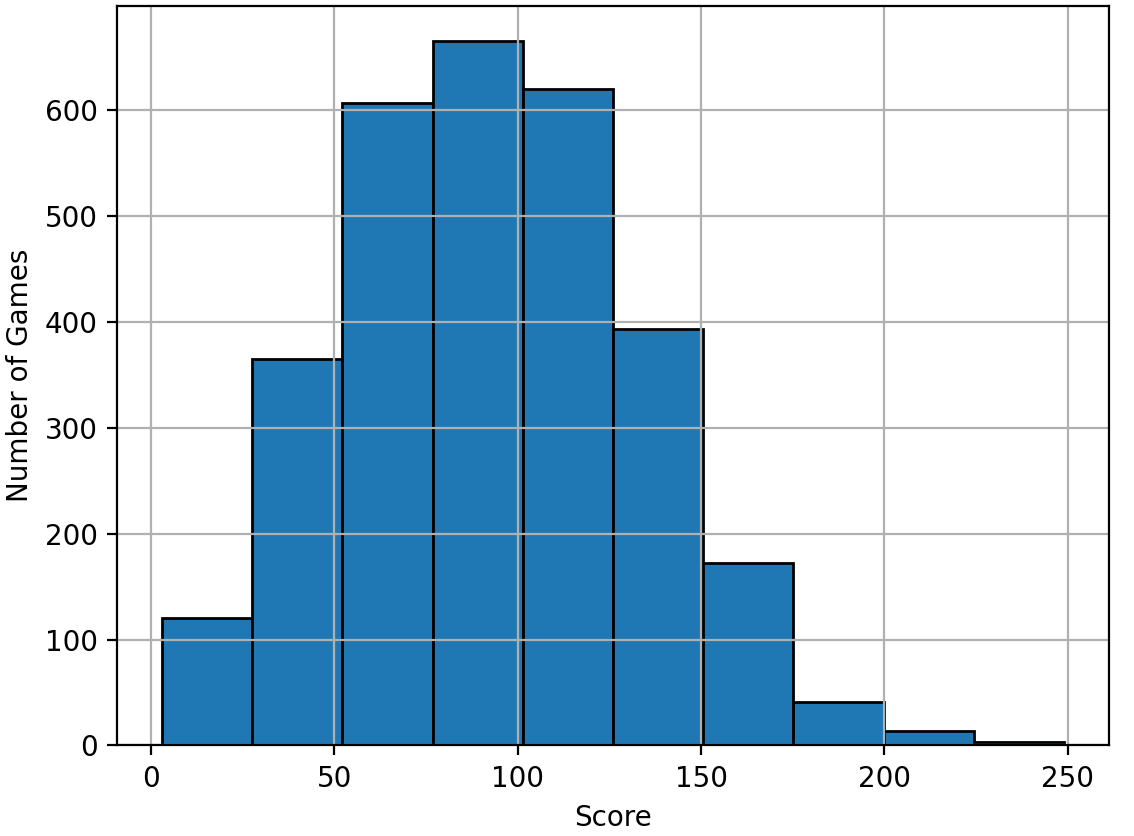
\includegraphics[width=0.58\linewidth]{Figures/histoneural.png} 
	\caption{Histogram rezultata izvježbane umjetne neuronske mreže s izbjegavanjem opasnosti kroz 3000 instanci igre}
	\label{slk:neural_histograph}
\end{figure}

Iz priloženih histograma vidljivo je da je raspored rezultata prilično podjednak, što znači da obje tehnike ostvaruju sličan rezultat. Čak su i sakupljeni najveći postignuti rezultati slični, 329 za neuronsku mrežu te 315 za heuristiku. No umjetna neuronska mreža s informacijama o praznim koncima doseže najveći rezultat od čak 526 bodova.



%--- ZAKLJUČAK / CONCLUSION ----------------------------------------------------
\chapter{Zaključak}
\label{pog:zakljucak}

U ovom radu promotrili smo igru Entanglement, te za nju konstruirali agente korištenjem heuristika promatrajući jednostavne tehnike za skupljanje što više bodova. Zatim su konstruirani i agenti koji koriste umjetne neuronske mreže, svaki prošireniji od prošlog te uspoređeni u nadi razvijanja agenta koji može postići bolji rezultat od čovjekovog.

Zbog pada točnosti neuronske mreže kod povećavanja ulaza, teško je istrenirati umjetnu neuronsku mrežu za igranje igre Entanglement jer svako stanje igre sadrži previše informacija, što vodi smanjenoj mogućnosti prilagođavanja mreže. Potrebno je pažljivo odabrati ulaze kako se to ne bi dogodilo.

Ako usporedimo opseg pravila heuristike i ulaza umjetne neuronske mreže, na temelju većeg prosječnog rezultata heuristika zaključujemo da one rade bolje. Tek kad se proširi opseg neuronske mreže, ona pokazuje bolji rezultat.

Sljedeći koraci nastavili bi s proširivanjem polja ulaza neuronske mreže, te isprobavanjem različitih varijanti nad postojećim ulazima. Također, zbog činjenice da sama sreća utječe na izgled svake pločice, isprobavanje agenata nad većim brojem igara povećalo bi i šansu za većim najboljim rezultatom.  



%--- LITERATURA / REFERENCES ---------------------------------------------------

% Literatura se automatski generira iz zadane .bib datoteke / References are automatically generated from the supplied .bib file
% Upiši ime BibTeX datoteke bez .bib nastavka / Enter the name of the BibTeX file without .bib extension
\bibliography{literatura}



%--- SAŽETAK / ABSTRACT --------------------------------------------------------

% Sažetak na hrvatskom
\begin{sazetak}
   Ovaj rad prati razvoj agenta za igranje igre entanglement. Opisana su pravila igre i korišteni program na koji se spajala logika agenta. Promatrane su neke jednostavne heuristike, te je tada konstruiran i poboljšan agent koji koristi umjetne neuronske mreže. U radu su opisani korišteni termini i struktura koda. Rezultati prikazani u obliku grafova, te međusobno uspoređeni. 

\end{sazetak}

\begin{kljucnerijeci}
  razvoj agenta; umjetna neuronska mreža; heuristike
\end{kljucnerijeci}


% Abstract in English
\begin{abstract}
	This thesis explains the development of an agent tasked to play the Entanglement online game. The rules of the game, as well as the program used for connecting the agent to the game's logic have been explained. The thesis presents some simple heuristics, and then the construction of an artifitial neural network agent trough different stages of development. Terms used and code structure are also described. The results are available in the form of graphs, and have been mutually compared.
\end{abstract}

\begin{keywords}
  agent development; heuristics; artifitial neural network
\end{keywords}


%--- PRIVITCI / APPENDIX -------------------------------------------------------

% Sva poglavlja koja slijede će biti označena slovom i riječi privitak / All following chapters will be denoted with an appendix and a letter
\backmatter




\end{document}
